
\chapter{Classification}
\label{ch:capitolo3}
Classification was performed on the available training set using three different algorithms: K-NN (\textit{K-Nearest Neighbours}), Naïve Bayes and Decision Trees.
For K-NN \textbf{and Naïve Bayes}, a portion of the training set (referred to as the validation set) was used to select the best hyperparameters \textbf{each} model.
The features used in K-NN and Naïve Bayes were normalized, as these models are sensitive to unscaled values.
In particular, a log-transformation and \textbf{SCRIVERE SE StandardScaler O MINMAX} were applied to data.
After training, the models were evaluated on the test set using standard performance metrics. 
The target variables chosen for this task are 2: \texttt{titleType}, and \texttt{has\_LowEngagement}.
These will be discussed in more detail in the corresponding sections below.

\section{Binary classification}\label{sec:binary_classification}
The binary target variable used in this task, \texttt{has\_LowEngagement}, was specifically defined for this purpose. 
It identifies records where the \texttt{numVotes} attribute is less than 100.\\

An analysis of semantically related features was run, in order to decide whether to discard any other feature.
\texttt{userReviewsTotal} showed a 75\% correlation with
\texttt{numVotes}, while \texttt{criticReviewsTotal} has 67\% correlation.
Despite the similarity in correlation
values, \texttt{userReviewsTotal} was deemed too semantically similar to \texttt{numVotes}, whereas
\texttt{criticReviewsTotal} was considered to provide distinct and complementary information.
The correlation value of the second considered not sufficiently high to make the problem trivial.\\

An important aspect of the chosen binary classification task is the class imbalance, with 10287 records
classified as \textit{Low Engagement} and 4668 as \textit{High Engagement} in the training set.
This imbalance was taken into account during model training and evaluation, with a focus on
macro-averaged F1-score to mitigate its impact on the results.\\

\subsection{K-NN}


\subsection{Naïve Bayes}


\subsection{Decision Trees}
For explainability purposes, features were not normalized nor transformed for the Decision Tree model,
as it does not require such preprocessing because it's not based on distance measures, but rather on
decision thresholds.\\

To identify the optimal hyperparameters, a Randomized Search was performed
using Repeated Stratified 5-Fold Cross-Validation with 10 repeats on the training set, optimized for
the macro-averaged F1-score.
The best configuration found used Gini index as the splitting criterion,
a maximum tree depth of 26, and a minimum of 3 samples per leaf.
Post-pruning did not yield any performance improvement and was therefore not applied.
The obtained decision tree is shown in figure~\ref{fig:binary_dt}.
\begin{figure}[H]
    \centering
    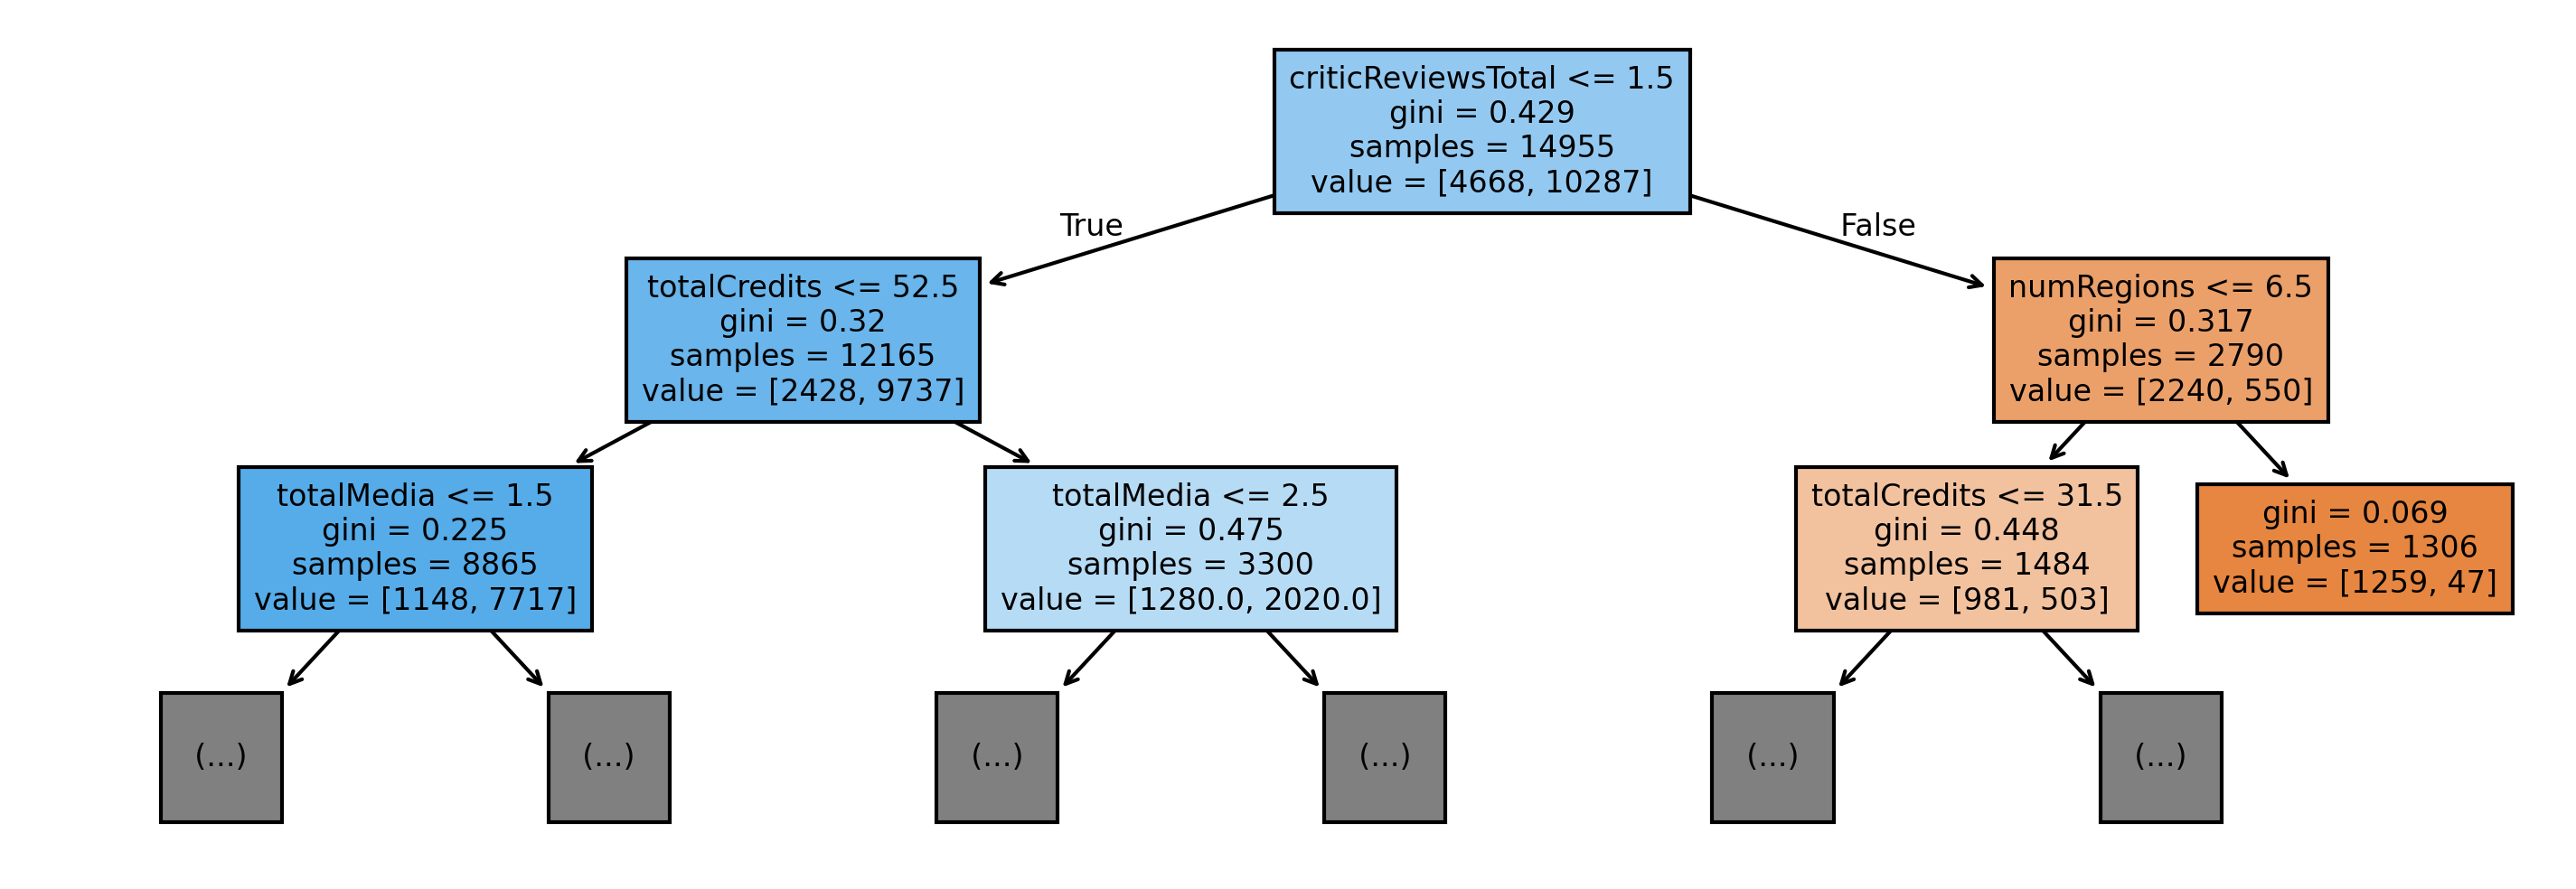
\includegraphics[width=0.8\linewidth]{plots/binary_dt.png}
    \captionsetup{justification=centering, width=0.9\linewidth}
    \caption{Decision Tree for binary classification}
    \label{fig:binary_dt}
\end{figure}

Unsurprisingly, the most important feature for the model was \texttt{criticReviewsTotal},
which amounted to 0.6 in the feature importance ranking. The following other 3 more important
features were \texttt{totalCredits} (0.15), \texttt{totalMedia} (0.10) and \texttt{numRegions} (0.09).
These four features take up around 93\% of the total feature importance, and are all present in the first
two splits shown in the Decision Tree.\\
% Classification performance is summarized in Table~\ref{tab:binary_classification_report}.

% \begin{table}[H]
%     \centering
%     \begin{tabular}{lcccc}
%         \toprule
%         \bf{Class} & \bf{Precision} & \bf{Recall} & \bf{F1-score} & \bf{Support} \\
%         \midrule
%         \bf{Low engagement} & 0.86 & 0.90 & 0.88 & 3416 \\
%         \bf{High engagement} & 0.75 & 0.69 & 0.72 & 1561 \\
%         \midrule
%         \bf{Macro avg} & 0.81 & 0.79 & 0.80 & \\
%         \bf{Weighted avg} & 0.83 & 0.83 & 0.83 & \\
%         \midrule
%         % & & \textbf{Train} & \textbf{Test} & \\
%         % \midrule
%         \bf{ROC AUC} & & & 0.87 & \\
%         \bf{Accuracy}  &  & & 0.83 & \\
%         \bottomrule
%     \end{tabular}
%     \caption{Classification report for binary classification}
%     \label{tab:binary_classification_report}
% \end{table}
Train performance was overall similar to the test performance; in particular, the respective accuracies
were of 0.83 and 0.84, and macro-F1 scores were 0.82 and 0.80.
The \textit{High Engagement} class showed low Recall values (0.71 on train set, 0.68 on test set).
This might be a consequence of class imbalance, as well as poor separability of the two classes.
This assumption is further supported by the
Precision scores of the class (0.78 on train, 0.75 on test).

% \begin{figure}[H]
%     \begin{minipage}{0.58\textwidth}
        % Figure~\ref{fig:conf_matr_binary_dt} shows the confusion matrix for the obtained
        % Decision Tree, with results regarding the test set.
        % As can be seen, a significant number of \textit{High Engagement} records was misclassified,
        % leading to a low Recall for that class.
        % This might be a consequence of class imbalance, as well as the possible presence
        % of noise in the data. It's also possible that the two classes are not well separated, leading
        % the model to prioritize the predominant class.\\
%     \end{minipage}
%     \hfill
%     \begin{minipage}{0.38\textwidth}
%         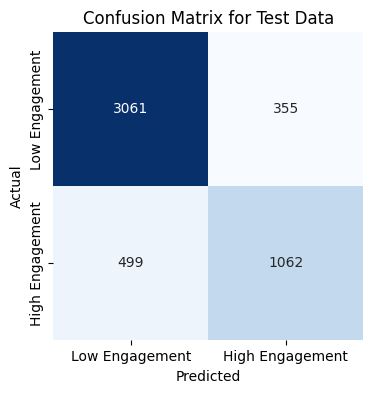
\includegraphics[width=\linewidth]{plots/binary_dt_confusion_matrix.png}
%         \captionsetup{justification=centering, width=0.9\linewidth}
%         \caption{Confusion matrix for binary classification}
%         \label{fig:conf_matr_binary_dt}
%     \end{minipage}
% \end{figure}

\subsection{Model Comparison}

\section{Multiclass classification}\label{sec:multiclass_classification}
Among the multiclass features in the training set, \texttt{titleType} was selected as the target variable
for this task, due to its relevance within the dataset. Because of their strong correlation with
\texttt{titleType}, the features \texttt{canHaveEpisodes} and \texttt{is\_Short} were excluded from the
feature set. Furthermore, since the primary imputation method for missing values in \texttt{runtimeMinutes}
relied on information from the target variable, these values were re-imputed to avoid data leakage.
Specifically, missing entries were filled by sampling from the overall distribution of
\texttt{runtimeMinutes}, without referencing \texttt{titleType}.\\

One final point to note is the imbalance in the target feature (previously shown in
figure~\ref{fig:titleType_distrib}), which was explicitly taken into account
during the design of the models. As for the binary classification task, macro-averaged F1-score was
a key metric for model evaluation, as it provides a balance between each class's precision and recall.



% This feature was created to impute the missing values of the original \texttt{runtimeMinutes} variable,
% but without using the median value according to the titleType. Instead, the missing values were imputed using the help of two variables: \texttt{canHaveEpisodes} and \texttt{is\_Short}
% (as one of the resulting variables of the multi-label one-hot encoding process of the \texttt{genres} attribute).
% In particular, 
% \textbf{SCRIVERE COME E' STATA IMPUTATA NO\_TT - con canhaveepisodes e is\_short preso dai generi}.
% This approach prevents a significant error, as it would be methodologically incorrect to use \texttt{titleType}-based 
% imputation for an attribute when \texttt{titleType} itself is the target variable to predict.
\subsection{K-NN}
\subsection{Naïve Bayes}
\subsection{Decision Trees}
% \begin{table}[H]
%     \centering
%     \begin{tabular}{lcccc}
%         \toprule
%         \bf{Class} & \bf{Precision} & \bf{Recall} & \bf{F1-score} & \bf{Support} \\
%         \midrule
%         \bf{movie}         & 0.85 & 0.88 & 0.87 & 1877 \\
%         \bf{short}         & 0.92 & 0.94 & 0.93 & 766 \\
%         \bf{tvEpisode}     & 0.89 & 0.92 & 0.90 & 1599 \\
%         \bf{tvMiniSeries}  & 0.51 & 0.35 & 0.41 & 81 \\
%         \bf{tvMovie}       & 0.36 & 0.29 & 0.32 & 299 \\
%         \bf{tvSeries}      & 0.89 & 0.94 & 0.91 & 447 \\
%         \bf{tvShort}       & 0.00 & 0.00 & 0.00 & 16 \\
%         \bf{tvSpecial}     & 0.32 & 0.12 & 0.18 & 49 \\
%         \bf{video}         & 0.55 & 0.46 & 0.50 & 250 \\
%         \midrule
%         \bf{Macro avg}     & 0.59 & 0.54 & 0.56 & 5384 \\
%         \bf{Weighted avg}  & 0.82 & 0.84 & 0.83 & 5384 \\
%         \midrule
%         \bf{Accuracy}      &      &      & 0.84 & 5384 \\
%         \bottomrule
%     \end{tabular}
%     \caption{Classification report for multiclass classification (\texttt{titleType})}
%     \label{tab:multiclass_classification_report}
% \end{table}




\subsection{Model Comparison}
Because of class imbalance, for evaluation purposes,
macro-averaged F1-score was heavily considered.